\documentclass[a4paper,11pt,reqno]{amsart}
\usepackage{M67tds}

\begin{document}

\hautdepage{TD1: Titre du td}

% ==================================
\section{Le plan euclidien}
% ==================================

\begin{convention}
  Le plan cartésien $\R^2$ est noté $\ens{P}$. Il est muni de la distance euclidienne
  \[
    d(A,B)=\sqrt{(x_B-x_A)^2+(y_B-y_A)^2}
  \]
  pour tous $A=(x_A,y_A)$, $B=(x_B,y_B)$ dans $\ens{P}$.
\end{convention}


%-----------------------------------
\begin{exo} (Projeté orthogonal)

  Soient $A$ un point et $\ens{D}$ une droite du plan.
  \begin{enumerate}
     \item Montrer qu'il existe une unique droite perpendiculaire\footnote{Deux droites sont perpendiculaires si elles se coupent en formant un angle droit, ou encore si tout vecteur directeur de l'une est orthogonal à tout vecteur directeur de l'autre.} à $\ens{D}$ passant par $A$. On appelle \emph{projeté orthogonal} de $A$ sur $\ens{D}$ le point d'intersection de $\ens{D}$ et sa perpendiculaire passant par $A$.
     \item Exprimer les coordonnées du projeté $H$ en fonction de celles de $A$ et d'une équation de $\ens{D}$.
     \item Montrer que $d(A,H)\leqslant d(A,M)$ pour tout $M \in \ens{D}$, avec égalité si et seulement si $M=H$.
  \end{enumerate}
\end{exo}


%-----------------------------------
\begin{exo} (Inégalité triangulaire)

  Soient $A,B,C$ trois points du plan deux à deux distincts.
  \begin{enumerate}
    \item Montrer que si $A$, $B$ et $C$ sont alignés dans cet ordre (c.-à-d. si $B \in [AC]$) alors $d(A,B)+d(B,C)=d(A,C)$.
    \item En considérant le projeté orthogonal de $B$ sur $(AC)$, montrer que
    \[
      d(A,C) \leqslant d(A,B)+d(B,C),
    \]
    avec égalité si et seulement si $B \in [AC]$.
    \item Retrouver cette inégalité (et le cas d'égalité) en rappelant que $d(A,B)^{2}=\vv{AB}\cdot\vv{AB}$.
    \item Étudier l'intersection des deux cercles $\ens{C}(A_1,r_1)$ et $\ens{C}(A_2,r_2)$.
  \end{enumerate}
\end{exo}


%-----------------------------------
\begin{exo} (Triangle rectangle)

  Soit $\tri ABC$ un triangle rectangle en $A$, et soit $H$ le pied de la hauteur issue de $A$ (autrement dit, le projeté orthogonal de $A$ sur $(BC)$).  Montrer que
  \[
    BA^2=BH \cdot BC,\ \ CA^2=CH \cdot CB,\ \ AH^2=BH \cdot CH.
  \]
  \begin{indication}
    On pourra utiliser la trigonométrie vue au collège.
  \end{indication}
\end{exo}


%-----------------------------------
\begin{exo} (Tout triangle est isocèle)

  On donne ici un argument pour établir que tout triangle est isocèle (dû à W.W. Rouse Ball).
  Soit $\tri ABC$ un triangle quelconque. Soit $D$ le point d'intersection de la bissectrice de l'angle $\widehat{BAC}$ avec la médiatrice du côté opposé $[BC]$. Soient $E,F$ et $G$ les projetés orthogonaux de $D$ sur $[BC]$,$[AB]$ et $[AC]$.\\[-.7\baselineskip]
  \sidebyside{.70}{
    \begin{enumerate}
      \item Montrer que $DF=DG$ et $AF=AG$.
      \item Montrer que $DB=DC$, puis que $FB=GC$.
      \item En déduire que $ABC$ est isocèle, puis qu'il est équilatéral.
      \item Comment expliquer cela?
    \end{enumerate}
  }{
    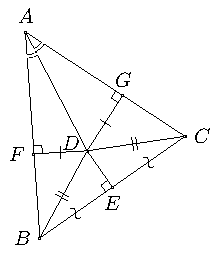
\includegraphics[width=35mm]{M67_2017-18_TD1_img1}
  }
\end{exo}


%-----------------------------------
\begin{exo} (Triangle isocèle)

  Soit $\tri ABC$ un triangle isocèle avec $AB=AC > BC$. On porte des points $D$ sur $(AB)$, avec $B$ entre $A$ et $D$, et $E$ sur $(BC)$, avec $C$ entre $B$ et $E$, et tels que $BD=CE=AB-BC$.

  Montrer que $\tri ADE$ est un triangle isocèle.
\end{exo}


% ==================================
\section{Nombres constructibles à la règle et au compas}
% ==================================


\begin{convention}\small
  Un point $M$ du plan est constructible en un pas (sous-entendu à la règle et au compas) à partir d'un ensemble de points $S=\{A_1,\ldots,A_k\}$ si c'est un point d'intersection
  \begin{itemize}
    \item de deux droites distinctes passant chacune par deux points de $S$,
    \item ou d'une droite passant par deux points distincts de $S$ et d'un cercle centré en un point de $S$ et passant par un autre point de $S$,
    \item ou de deux cercles distincts centrés en des points de $S$ et passant par des points de $S$.
  \end{itemize}

  Un point $M$ est dit \emph{constructible à partir de $S$} s'il est constructible en un nombre fini de pas, c'est à dire s'il existe $M_1,M_2,\ldots,M_{r-1},M_r=M$ tels que $M_{i+1}$ est constructible en un pas à partir de $S \cup \{M_1,\ldots,M_{i}\}$ pour tout $i=1,\ldots,r-1$.

  Un point \emph{constructible} est un point constructible à partir de $O=(0,0)$ et $I=(1,0)$.

  Enfin, un nombre réel $x$ est un \emph{nombre constructible} si le point $(x,0)$ est constructible. Plus généralement, un nombre complexe $z=x+iy$ avec $x,y \in \R$ est constructible si le point $(x,y)$ est constructible. En utilisant l'identification habituelle entre $\C$ et $\R^2$,  cela revient à dire que le point d'affixe $z$ est constructible.
\end{convention}


%-----------------------------------
\begin{exo} (Premières constructions)

  Tracer à la règle et au compas les figures suivantes:
  \begin{enumerate}
    \item le symétrique d'un point $A$ par rapport à un point $O$,
    \item le milieu d'un segment $[AB]$,
    \item la médiatrice d'un segment $[AB]$,
    \item la parallèle à une droite $(AB)$ passant par un point donné,
    \item la perpendiculaire à une droite $(AB)$ passant par un point donné (attention aux cas particuliers),
    \item la bissectrice d'un angle $\widehat{BAC}$,
    \item le centre d'un cercle donné,
    \item le cercle de centre $A$ et de rayon $BC$ (ainsi on peut ajouter dans la définition de point constructible les cercles centrés en un point déjà construit et de rayon égal à la distance entre deux points déjà construit, ce qui revient à reporter l'écartement du compas).
  \end{enumerate}
\end{exo}

\end{document}
